\documentclass[../validierung.tex]{subfiles}
\graphicspath{{./coverage/}{./5_statistik/coverage/}}
\begin{document}

\section{Test-Überdeckung}
	Für die Test-Überdeckung wurde das Plugin \gls{dotcover} verwendet.

	Im folgenen sind die ermittelten Überdeckungen aufgelistet:
	In Prozent und als Verhältnis \quote{nicht abgedeckte Code-Blöcke} zu \quote{Code-Blöcke insgesamt}.
	\subsection{Karl}
		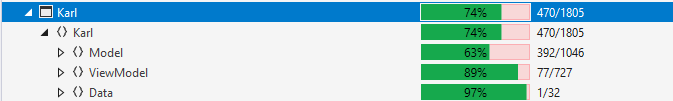
\includegraphics[width=\textwidth]{karl.png}
			\subsubsection{Model}
				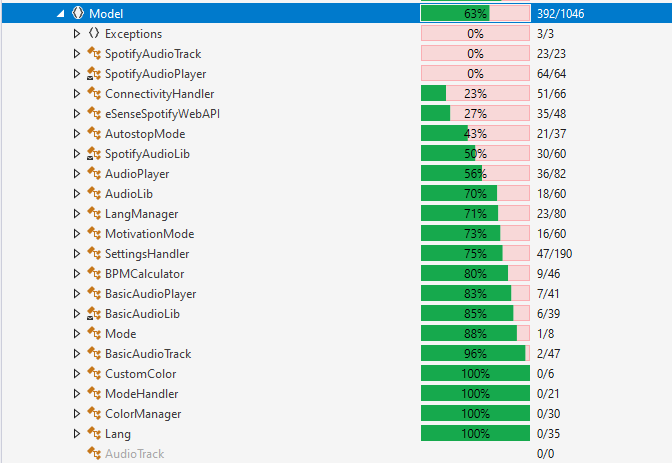
\includegraphics[width=\textwidth]{model.png}
			\subsubsection{ViewModel}
				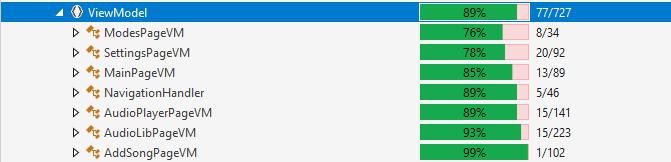
\includegraphics[width=\textwidth]{vm.png}
			\subsubsection{Data}
				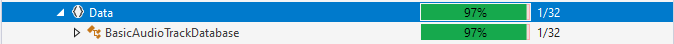
\includegraphics[width=\textwidth]{data.png}
	\subsection{EarableLibrary}
		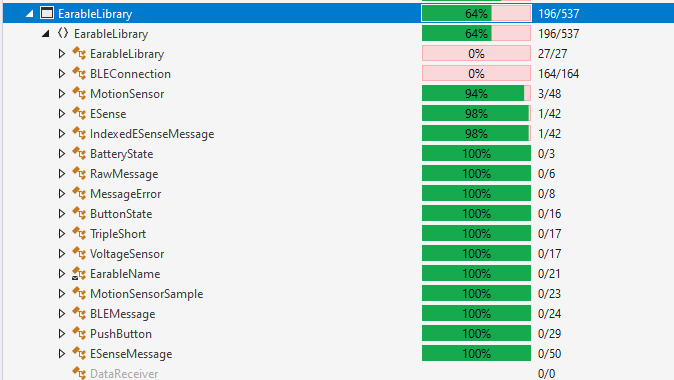
\includegraphics[width=\textwidth]{ear.png}
	\subsection{StepDetectionLibrary}
		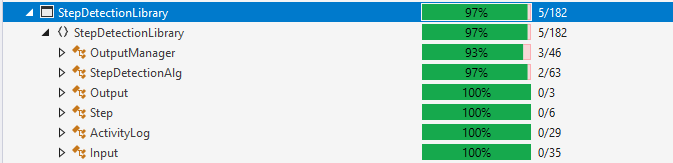
\includegraphics[width=\textwidth]{step.png}

\end{document}
